\documentclass{IEEEcsmag}

\usepackage[colorlinks,urlcolor=blue,linkcolor=blue,citecolor=blue]{hyperref}

\usepackage{upmath}

\jvol{XX}
\jnum{XX}
\paper{8}
\jmonth{May/June}
\jname{Security \& Privacy}
\pubyear{2019}
\newtheorem{theorem}{Theorem}
\newtheorem{lemma}{Lemma}

\setcounter{secnumdepth}{0}

\begin{document}

\sptitle{Department: Head}
\editor{Editor: Name, xxxx@email}

\title{Cyber Assured Systems Engineering at Scale}

\author{Darren Cofer, Isaac Amundson, Junaid Babar, David Hardin, Konrad Slind}
\affil{Collins Aerospace}

\author{S. B. Author, Jr.}
\affil{Second Affiliation}

\author{T. C. Author, III}
\affil{Third Affiliation}

\markboth{Department Head}{Paper title}

\begin{abstract}
Abstract text goes here. This single paragraph ($\le$50 words) summarizes the significant aspects of the manuscript. Often it indicates whether the manuscript is a report of new work, a review or overview, or a combination of thereof. Do not cite references in the abstract. Papers must not have been published previously, must fit into the theme of an open Call for Papers, and must be targeted toward the general technical reader. 
\end{abstract}

\maketitle


\chapterinitial{The introduction} should provide background information (including relevant references) and should indicate the purpose of the manuscript. Cite relevant work by others, including research outside your company. Place your work in perspective by referring to other research papers. Inclusion of statements at the end of the introduction regarding the organization of the manuscript can be helpful to the reader.

Darren, David?
%Introduction
\chapterinitial{Aerospace systems engineers} are currently given few
development tools to understand and mitigate 
potential cybersecurity vulnerabilities.  Typically, they must rely on
process-oriented checklists and guidelines. Cyber vulnerabilities
are often discovered during penetration testing late in the
development process. Worse yet, they may be discovered
only after the product has been fielded, necessitating extremely
expensive and time-consuming remediation. This is not a
sustainable development model.

Fortunately, formal methods tools have advanced to the point that they can 
be used to address cybersecurity and cyber-resiliency design challenges
on real high-assuance systems at industrial scale.  
Our application domain is avionics and aerospace systems in general.  
They are typically large, real-time cyberphysicial systems with the added 
complexities of performing safety-critical tasks and being exposed to 
a wide variety of cyber threats.  Furthermore, they are subject 
to intense regulatory scrutiny due to the certification requirements of this domain. 

In previous work on the High-Assurance Cyber Military Systems (HACMS) project \cite{HACMS}
we demonstrated that formal methods could be used to dramatically improve the 
cyber-resiliency of real aircraft, including an unmanned military helicopter.  Our current
work is focused on automating the capabilities that we prototyped in the HACMS project
and extending the reach and scale of the formal methods design and verification approach.  

To this end, we have developed a model-based systems engineering (MBSE) 
environment that allows engineers to address a range of properties and 
manage system complexity through compositional analysis, integrating formal methods
at all levels of the design process.  MBSE processes use model as the primary vehicle for 
communication among the parties tasked with designing the system and as the primary 
design artifacts for requirements, verification, and code generation.  

Our tools are based on the 
Architecture Analysis and Design Language (AADL) and extend the Open Source
AADL Tool Environment (OSATE) \cite{OSATE}.  The tools are specifically designed 
to bridge the gap between a user-level modeling language accessible to systems 
engineers and the highly specialized, formally verified code that implements the operating system (OS)
kernel and other high-assurance components.   

By using these tools to build real avionics systems, we show 
that current formal methods tools are practical, effective, and scalable to significant 
high-assurance applications in the aerospace industry.  


\section{INNOVATIONS}
Darren
%Innovations

MBSE environment for high-assurance systems, providing access to FM tools at every level, integrating assurance evidence for co-evolving design and associated evidence.

\begin{enumerate}
\item Semi-automated architectural design patterns to address cyber-resiliency requirements, including synthesis of high-assurance components
\item MBSE environment that leverages seL4 security guarantees and makes this accessible
\item Co-evolution of system design and certification evidence/artifacts, organized by assurance argument
\item Integration of formal methods throughout the workflow (or is this part of one of the other innovations?)
\end{enumerate}

As part of the DARPA Cyber Assured Systems Engineering (CASE) program,
our team has developed design, analysis, and verification
tools that enable systems engineers to design-in cyber-resiliency
for complex cyber-physical systems. We have produced a prototype
Model-Based Systems Engineering (MBSE) environment called
BriefCASE which is based on the Architecture Analysis and Design
Language (AADL). BriefCASE extends the Open Source AADL
Tool Environmnet (OSATE) to add new design, analysis, and code
generation capabilities targeted at building cyber-resilient systems.
BriefCASE provides access to two analysis tools (GearCASE 
and DCRYPPS) that can examine AADL models to detect potential
cyber vulnerabilities and suggest requirements for mitigation.
A library of architectural transforms guides systems engineers
through automated model transformations that modify the
architecture to address these requirements, possibly inserting new
high-assurance components into the system. Implementations for
these new high-assurance components are synthesized from formal
specifications using the Semantic Properties for Language and
Automata Theory (SPLAT) tool. Formal verification that the
transformed system model satisfies its cyber requirements is accomplished
via model checking using the Assume Guarantee Reasoning
Environment (AGREE). Cyber-resilient code implementing the
verified model is automatically generated using the High Assurance
Modeling and Rapid Engineering for Embedded Systems (HAMR)
toolkit. If desired, this code can be targeted to the formally
verified seL4 secure microkernel.
A novel aspect of our approach is the use of an assurance argument
embedded in the architecture model itself to capture and
document the design decisions made during this process, along
with associated rationale.


\section{MOTIVATION}
Eric?
%Motivation
\begin{figure*}
	\begin{center}
	  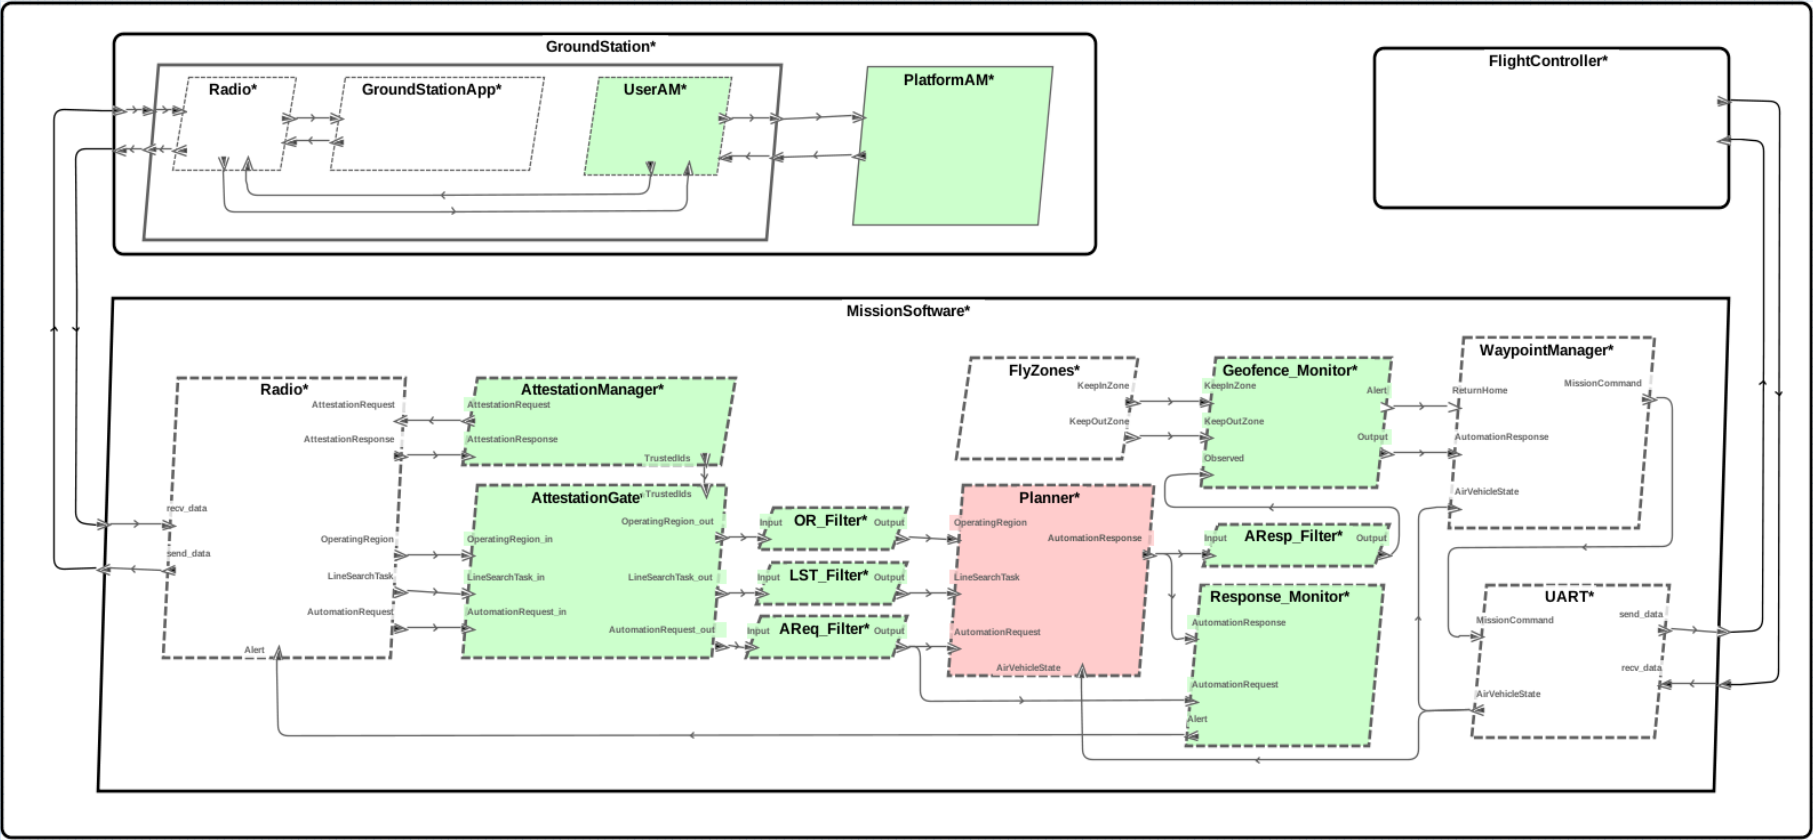
\includegraphics[width=\textwidth]{./figs/sw-hardened.png}
  \end{center}
	\caption{Cyber-resilient software architecture for UAV surveillance system. MAKE NAMES BIGGER} 
	\label{fig:sw-hardened} 
\end{figure*}

\figref{fig:sw-hardened} is a model-based design in the AADL OSATE tool of a cyber-hardened software
system for an autonomous UAV for surveillance.
The original \emph{unhardened system} consists of four components: the radio to communicate with a
remote ground
station (\emph{Radio}), mission planning automation (\emph{UxAS}), waypoint metering
(\emph{WaypointManager}), and a UART to talk to the flight controller (\emph{UART}).

\briefcase\ integrates four key formal methods in the model-based engineering workflow:
assume-guarantee verification (\agree), synthesis of high-assurance components (\splat), synthesis
of inter-component communication (\hamr), and the \selFour\ verified microkernel.
Each component in the unhardened system, and the interface for the top-level software component, is
formally specified with an AGREE contract stating assumptions on inputs and guarantees on outputs
under the assumptions.
\agree\ proves the unhardened implementation obeys the composition of these contracts. 

Cyber-threat analysis (GearCASE and DCRYPPS) identifies the ground station and the planning
automation services as primary cyber threats to the system.
Seven new cyber requirements are added to the unhardened system that require ground station
certification, message integrity, and monitoring.
The existing contracts in the unhardened system are strengthened to reflect these new requirements.
\agree\ proves the unhardened system under these contracts fails verification. 

Design engineers use \briefcase\ to transform the unhardened system to that in
\figref{fig:sw-hardened} by inserting high-assurance components.
\emph{Attestation} proves the identity of trusted ground stations (\emph{AttestationManager}) while
the \emph{gate} only passes messages from trusted sources (\emph{AttestationGate}).
\emph{Filters} only pass well-formed messages (\emph{OR\_Filter}, \emph{LST\_Filter},
\emph{AReg\_Filter}, and \emph{AResl\_Filter}).
\emph{Monitors} alert to suspicious behavior such as missions that enter keep-out zones or leave
keep-in zones (\emph{Geofence\_Monitor}) or unrequested missions from automation
(\emph{Response\_Monitor}).
The interface behavior of these high-assurance components, with the exception of attestation, is
specified with assume-guarantee contracts (e.g., a filter makes no assumptions on input and only
passes input that is well-formed).
\agree\ proves the hardened system ensures the added cyber requirements.

The \selFour\ target platform requires a static schedule that is provided in the model.
A transformation on the \agree\ contracts incorporates that schedule into the verification model.
\agree\ proves the scheduled hardened system also ensures cyber requirements.
The model is further refined to move the attestation and mission planning services into separate
virtual machines inside the microkernel.

\resolint\ certifies the hardened model is ready for synthesis.
\splat\ synthesizes high-assurance components from their \agree\ contracts to the target platform.
It includes proof certificates that the binaries have assumptions that are no stronger than those on
the original contracts and guarantees that are no weaker than those on the original contracts (e.g.,
safe substitution).
\hamr\ synthesizes all the inter-component communication primitives from the AADL model.
That synthesis includes a proof certificate that the resulting communication channels defined in
\selFour\ are only those defined in the AADL model.

\resolute\ builds an assurance case for the entire system.
That assurance case includes evidences for every requirement including proof certificates from
\agree, \splat, and \hamr.


\section{BRIEFCASE WORK FLOW}
Darren
%Work Flow

%Describe the BriefCASE work flow and tools.

% Copied from DESTION paper
The BriefCASE environment provides systems engineers with a workflow and tool support for developing
products with inherent cyber-resiliency. 
\remove{In this section we provide an overview of the design, analysis, and code generation tools and how they can be used
to implement high-assurance systems.  
}

%BriefCASE is predicated on an MBSE process, in which models are the primary vehicle for
%communication and understanding among the parties tasked with designing the system. Furthermore,
%MBSE models are the primary design artifacts used for analysis, verification, testing, and code
%generation.
The  workflow starts with the development of a baseline AADL model of the system architecture
focusing on the desired functionality. This model can be analyzed using any of the existing AADL 
tools (e.g., resource usage, information flow, latency) to determine whether it is acceptable.
BriefCASE integrates additional tools that analyze the architecture model for cybersecurity vulnerabilities and
generate requirements that, when addressed, will mitigate those vulnerabilities.
These requirements are imported into the model and may be addressed using a 
collection of automated model transforms. As requirements are addressed in the design, an assurance case is updated with
corresponding evidence, computed directly from the model or by supporting analysis tools.  
Code implementing new high-assurance components as well as communication and execution infrastructure
is generated from the model along with associated assurance evidence.  

The following sections describe each step of the workflow in more detail. 

%development process outputs, necessary
%to support the claim. In this manner, the assurance case is co-developed alongside the system
%design, and can be automatically evaluated throughout development.


\subsection{Requirements}
Isaac, Junaid

\subsection{Cyber Transforms}
Isaac

\subsection{High Assurance Component Synthesis}
Konrad, Eric, Junaid

\subsection{Remote Attestation}
Perry

\subsection{Compositional Analysis}
Isaac, Junaid

\subsection{Information Flow Analysis}
John H

\subsection{Real-Time Scheduling}
John S

\subsection{Infrastructure Code Generation}
John H

\subsection{Secure Microkernel}
Corey

\subsection{Assurance Case}
Isaac

\section{AIRCRAFT APPLICATION}
David, Darren?

Describe how we have used the BriefCASE tools to add new functionality to the CAAS architecture.  

\section{CONCLUSION}

The manuscript should include a conclusion. In this section, summarize what was described in your paper. Future directions may also be included in this section. Authors are strongly encouraged not to reference multiple figures or tables in the conclusion; these should be referenced in the body of the paper.

\section{ACKNOWLEDGMENT}

This work was funded by DARPA contract HR00111890001. The
views, opinions and/or findings expressed are those of the author
and should not be interpreted as representing the official views or
policies of the Department of Defense or the U.S. Government.


\begin{thebibliography}{1}

\bibitem{AA1}
G. M. Amdahl, G. A. Blaauw, and F. P. Brooks, ``Architecture of the IBM System/360,'' {\it IBM J. Res. \& Dev}., vol. 8, no. 2, pp. 87--101, 1964. (journal)

\bibitem{BB1}
IBM Corporation, IBM Knowledge Center - IBM Secure Service Container (Secure Service Container). [Online]. Available: {https://www.ibm.com/support/\break knowledgecenter/en/HW11R/com.ibm.hwmca.kc\_se.doc/\break introductiontotheconsole/wn2131zaci.html} (URL)

\bibitem{CC1}
J. Williams, ``Narrow-band analyzer,'' PhD dissertation, Dept. of Electrical Eng., Harvard Univ., Cambridge, MA: 1993. (Thesis or dissertation)

\bibitem{DD1}
J. M. P. Martinez, R. B. Llavori, M. J. A. Cabo, et al., ``Integrating data warehouses with web data: A survey,'' {\it IEEE Trans. Knowledge and Data Eng}., preprint, Dec. 21, 2007, doi:10.1109/TKDE.2007.190746. (PrePrint)

\bibitem{EE1}
W.-K. Chen, {\it Linear Networks and Systems}, Belmont, CA: Wadsworth, pp. 123--135, 1993. (book)

\bibitem{FF1}
S. P. Bingulac, ``On the compatibility of adaptive controllers,'' {\it Proc. Fourth Ann. Allerton Conf. Circuits and Systems Theory}, pp. 8--16, 1994. (conference proceedings)\vadjust{\vfill\pagebreak}

\bibitem{GG1}
K. Elissa, ``An overview of decision theory,'' unpublished. (Unpublished manuscript)

\bibitem{HH1}
R. Nicole, ``The last word on decision theory,'' {\it J. Computer Vision}, submitted for publication. (Pending publication)

\bibitem{II1}
C. J. Smith and J. S. Smith, Rocky Mountain Research Laboratories, Boulder, CO, personal communication, 1992. (Personal communication)
\end{thebibliography}


\begin{IEEEbiography}{First A. Author}{\,}current employment (is
currently with XYZ Corporation, New York, NY, USA). Author's latest degree received or which he/she is currently pursuing (He received the B.S. degree and the M.S. degree...."). Author's research interest. Association with any official journals or conferences; major professional and/or academic achievements, i.e., best paper awards, research grants, etc.; any publication information (number of papers and titles of books published). Author membership information, e.g., is a member of the IEEE and the IEEE Computer Society, if applicable, is noted at the end of the biography. Biography is limited to single paragraph only (He is a member of IEEE, etc.). All biographies should be limited to one paragraph, five to six sentences, consisting of the following: (e.g., ``Dr. Author received a B.S. degree and an M.S. degree $\ldots$.''), including years achieved; association with any official journals or conferences; major professional and/or academic achievements, i.e., best paper awards, research grants, etc.; any publication information (number of papers and titles of books published); current research interests; association with any professional associations. Author membership information, e.g., is a member of the IEEE and the IEEE Computer Society, if applicable, is noted at the end of the biography. Contact him/her at faauthor@xyz.com.
\end{IEEEbiography}

\begin{IEEEbiography}{Second B. Author, Jr.,}{\,}is with ABC Corporation, Bblingen, Germany. Ms. Author's biography appears here.  Contact him/her at sbauthor@abc.com.
\end{IEEEbiography}

\begin{IEEEbiography}{Third C. Author, III,}{\,}is with DEF Corporation, Tokyo, Japan. Dr. Author's biography appears here.  Contact him/her at tcauthor@def.com.
\end{IEEEbiography}

\end{document}

